%=================
\chapter{Sprint 2}
%=================


%------------------------
\section{Sprint Planning}
%------------------------
The first sprint resulted in a solid core for the utility. During the next sprint iteration, the core will be extended with more advanced functionality. After this sprint, the utility will have most of the functionalities it need to work in a real environment, and will probably be able to aid Thales in some of their operations.

Not yet understanding the complexity of all the requirements in the sprint backlog, the team ended in an uncertain person-hours estimate for some work objects. Time will show if we understood the complexity and assigned enough hours to implement it. The more complex, but not so critical functionalities will be part of sprint 3 and 4.   



\subsection{Duration}
%-----------------------
According to the work breakdown structure, \autoref{tab:wbs}, the planning meeting of the second sprint should have been conducted the 5th of October. After a request from the customer to see our planning for the second sprint at the weekly customer meeting, which was scheduled to be before our planning meeting the same day, we decided to advance the planning to the 4th of October. This is to maintain the good relationship to the customer and submit to their preference.

The sprint started with the planning meeting the 4th of October and our work started the following day. The sprint duration is 14 days, and will end the 18th of October with a review meeting.  

\subsection{Sprint Goal}
%-----------------------
The second sprint will build on the core created in the first sprint. During the sprint we will extend the functionality with more comprehensive and advanced features. Most of the requirements we intend to fulfill in this sprint had to be done subsequent to the first sprint, because the structure and design of the core had to be in place first. The requirements that are selected for this sprint is a natural advancement on the way to make the utility that the customer wants. 

One of the most crucial functions to work in a real environment, is the support for nested header-files. The handling of the \#include-statement gives the utility this feature. The goal of the sprint is to implement the \#include and mainly to have support for enums, bit streams, endianness and batch mode. 


\subsection{Back Log}
%-----------------------
The second sprint we will implement thirteen requirements. These are listed in Table
\ref{tab:sprint2req1} and Table \ref{tab:sprint2req2}.

\begin{table}[!ht] \small \center
\caption{Sprint 2 Requirements\label{tab:sprint2req1}}
\begin{tabularx}{\textwidth}{l l X c c}
	\toprule
	& & & \multicolumn{2}{c}{Hours} \\
	\cmidrule(r){4-5}
	\# & Req. & Description & Est. & Act. \\
	\midrule
	1 & FR1-B & Support members of type enums & \underline{ 6 } & 5 \\
	   &  & Implementation			   	& 3 & 2\\
	   &  & Testing - unit				   	& 1 & 1\\
	   &  & Testing - end to end			& 2 & 2\\
	\addlinespace
	2 & FR1-C & Support members of type structs & \underline{ 7 } & 3.5  \\
	   &  & Implementation			   	& 6 & 3\\
	   &  & Testing - unit				   	& 1 & 0.5\\
	\addlinespace
	3 & FR1-F & Detect structs with same name & \underline{ 3 } &  3.5  \\
	   &  & Implementation			   	& 2 & 2.5\\
	   &  & Testing - unit				   	& 1 & 1\\
	\addlinespace
	4 & FR2-B & Support display of structs within structs & \underline{ 11 } &  -  \\
	   &  & Implementation			   	& 5 & 2\\
	   &  & Testing - unit				   	& 2 & 1\\
	   &  & Testing - end to end			& 4 & 2\\
	\addlinespace
	5 & FR4-F & Support enumerated named values  & \underline{ 5 } &  -  \\
	   &  & Design				   	& 1 & 0.5\\	   
	   &  & Implementation			   	& 1 & 0.5\\
	   &  & Testing - unit				   	& 1 & -\\
	   &  & Testing - end to end			& 1 & 1.5\\
	   &  & User documentation		   	& 1 & -\\
	\addlinespace
	6 & FR4-G & Support for bit strings & \underline{ 10 } & 11.5 \\
	   &  & Design				   	& 2 & 2\\	   
	   &  & Implementation			   	& 3 & 6\\
	   &  & Testing - unit				   	& 2 & 1\\
	   &  & Testing - end to end			& 2 & 1\\
	   &  & User documentation		   	& 1 & 1.5\\
	\bottomrule
\end{tabularx}
\end{table}

\begin{table}[!ht] \small \center
\caption{Sprint 2 Requirements continued\label{tab:sprint2req2}}
\begin{tabularx}{\textwidth}{l l X c c}
	\toprule
	& & & \multicolumn{2}{c}{Hours} \\
	\cmidrule(r){4-5}
	\# & Req. & Description & Est. & Act. \\
	\midrule
	7 & FR1-E & Support members of type array & \underline{ 7 } & 11 \\
	   &  & Implementation			   	& 3 & 6\\
	   &  & Testing - unit				   	& 1 & 1\\
	   &  & Testing - end to end			& 3 & 4\\
	\addlinespace
	8 & FR4-E & Structs with various trailers & \underline{ 18 } & - \\
	   &  & Design				   	& 3 & 2\\
	   &  & Implementation			   	& 6 & 4\\
	   &  & Testing - unit				   	& 2 & 1\\
	   &  & Testing - end to end			& 5 & -\\
	   &  & User documentation		   	& 2 & -\\
	\addlinespace
	9 & FR4-B & Support for custom Lua configuration & \underline{ 14 } & - \\
	   &  & Design				   	& 2 & -\\
	   &  & Implementation			   	& 5 & -\\
	   &  & Testing - unit				   	& 1 & -\\
	   &  & Testing - end to end			& 4 & -\\
	   &  & User documentation		   	& 2 & -\\
	\addlinespace
	10 & FR4-D & Dissector ID & \underline{ 4 } & - \\
	   &  & Implementation			   	& 1 & 1\\
	   &  & Testing - unit				   	& 1 & 1\\
	   &  & User documentation 			& 2 & -\\
	\addlinespace
	11 & FR5-C & Endian handeling & \underline{ 11 } & - \\
	   &  & Implementation			   	& 5 & -\\
	   &  & Testing - unit				   	& 2 & -\\
	   &  & Testing - end to end			& 6 & -\\
	\addlinespace
	12 & FR6-C & Batch mode; folder support in the CLI & \underline{ 7 } & - \\
	   &  & Implementation			   	& 4 & -\\
	   &  & Testing - unit				   	& 2 & -\\
	   &  & User documentation			& 1 & -\\
	\addlinespace
	13 & FR4-C & Support custom handeling of specific data types & \underline{ 5 } & - \\
	   &  & Implementation			   	& 2 & -\\
	   &  & Testing - unit				   	& 1 & -\\
	   &  & Testing - end to end			& 1 & -\\
	   &  & User documentation			& 1 & -\\
	\midrule
	& & Total: & 108  & - \\
	\bottomrule
\end{tabularx}
\end{table}



\begin{table}[!ht] \small \center
\caption{Sprint 2 Timetable\label{tab:sprint2time}}
\begin{tabularx}{\textwidth}{X c c}
	\toprule
	& \multicolumn{2}{c}{Hours} \\
	\cmidrule(r){2-3}
	Description & Est. & Act. \\
	\midrule
	Design & 8 & -\\
	\addlinespace
	Implementation & 44 & - \\
	\addlinespace
	Testing & 46 & -\\
	\addlinespace
	Documentation & 10 & -\\
	\midrule
	Total: & 108 & - \\
	\bottomrule
\end{tabularx}
\end{table}

%----------------------
\subsection{User Stories}
%----------------------

\textbf{Requirement:} FR1-B: The utility must support members of type enum\\
\textbf{Who:} Administrator\\
\textbf{What:} The user wants the utility to support structs with members of type enum.\\
\textbf{How:} When the cparser module detects an enum member in a struct, the cparser should search in an enum dictionary and the enum member will be mapped to the correct value found in the dictionary. \\
\textbf{Result:} The utility supports members of type enum.\\




%----------------------
\section{System Design}
%----------------------
For sprint 2 the team decided to refactor some of the code in order to make it easier to read and to split the functionalities of the utility in such a way that it reduces coupling within the system.Some new functionality was also added on the parser side in order to get the utility to recognize the datatypes mentioned in the sprint 2 backlog. Other than that, there were no other changes or additions made to the design during sprint 2.

\subsection{Utility}
%--------------------
\autoref{fig:sp2:class} shows the class diagram the team made for sprint 2. The main differences from sprint 1 are the additions of new classes, extending the functionality of the utility so that the utility can handle more domplex header files than it could before. The developers also generalized some of the modules and used inheritance to support the re-use of code 
\begin{figure}[!htb]
	\center
	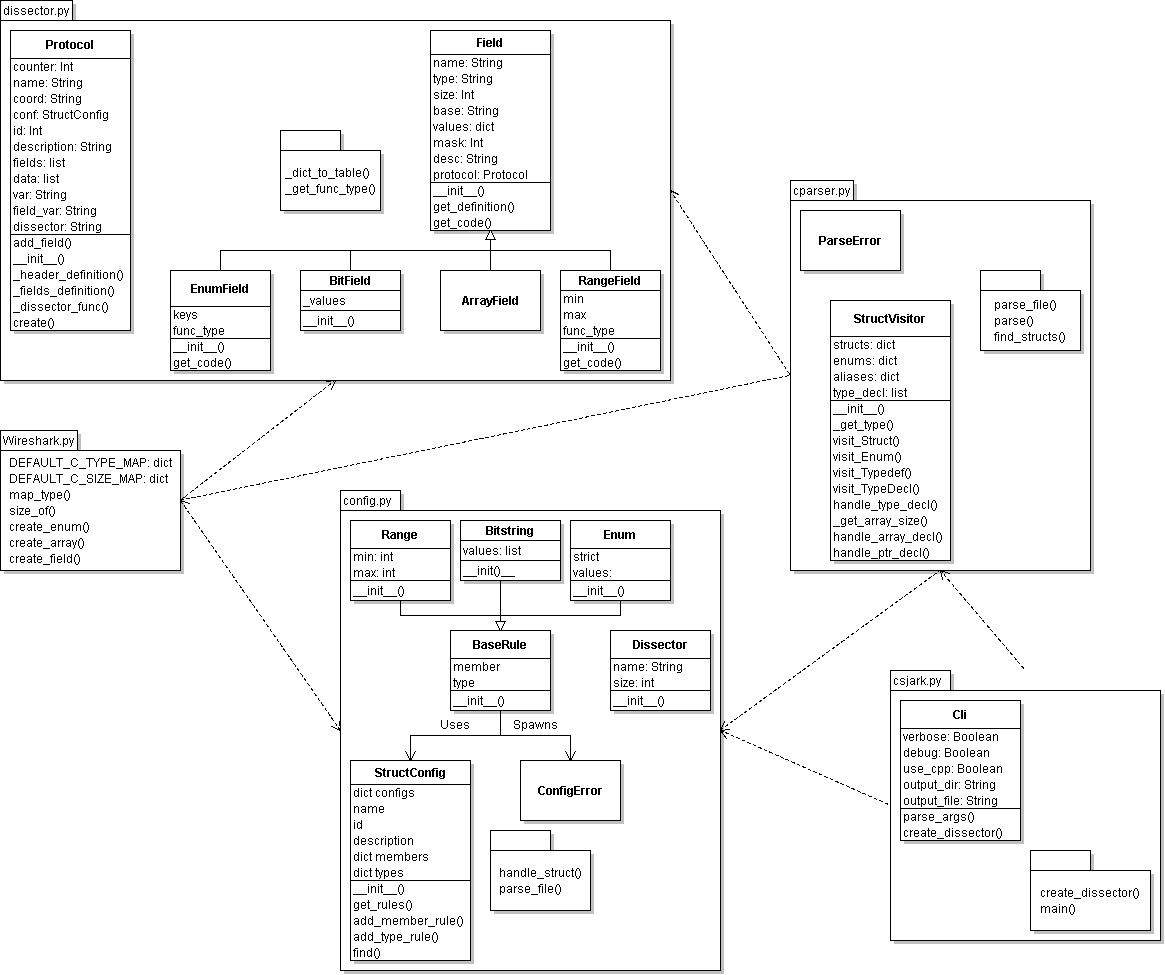
\includegraphics[width=\textwidth]{./sprints/img/class_diagram_s2}
	\caption{Class Diagram\label{fig:sp2:class}}
\end{figure}



%----------------------
\section{Implementation}
%----------------------

In the previous sprint we focused on creating a naive implementation of the 
utility. In this sprint the focus was on implementing data types for the 
C programming language and making it possible to configure more options on how 
the dissector will function. This section will cover the requirements 
implemented, how they were implemented and what the ''output'' looks like.

\subsection{Support Members of Type enum}
%----------------------
\label{sec:supportenum}
Enum is a type declaration in C, which specifies enumeration constants.  Enum 
is supported because it is a basic datatype in the C language. 
\autoref{code:cenum} shows an example of an enum in a C-header file. The 
Wireshark dissector will display the named value, making it 
easier to read, an example is shown in \autoref{fig:wscenum}. The red 
rectangle shows the enumerated named value.

\begin{figure}[ht]
	\center
	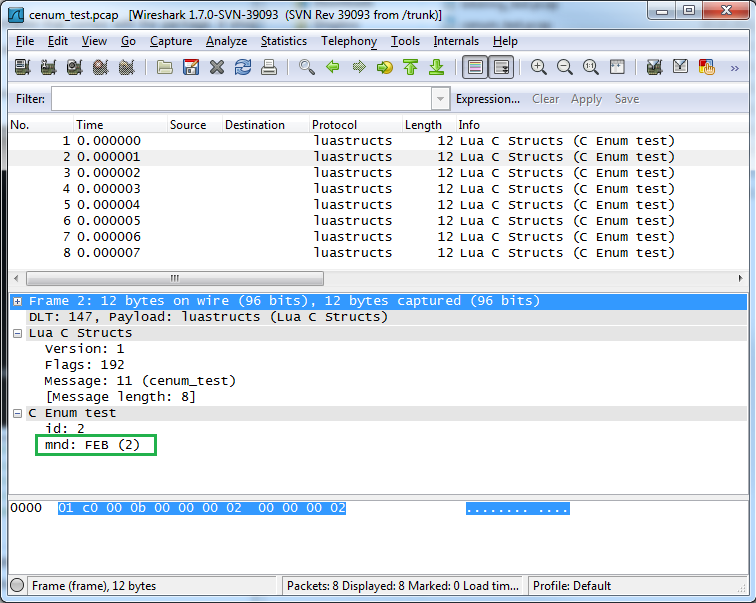
\includegraphics[width=\textwidth]{./sprints/img/wireshark_cenum}
	\caption{Enumeration in Wireshark\label{fig:wscenum}}
\end{figure}

\lstset{language=C,caption={Enum support},label=code:cenum}
\lstinputlisting[language=C]{./sprints/code/cenum_test.h}

\subsection{Support Members of Type Struct}
%----------------------
Structs are an important part of the C language, a struct declaration consists 
of a group of different fields, these fields can have any type, also struct. 
This was therefore an important requirement to implement. An example is shown 
in \autoref{code:structmember}.

\lstset{language=C,caption={Struct support},label=code:structmember}
\lstinputlisting[language=C]{./sprints/code/struct_member.h}

\subsection{Detect Structs with Same Name}
%----------------------
Two structs can have the same name, and therefore we needed a way of detecting it. 
If the parser finds two structs with the same name, an exception is 
raised, and the generation of the dissector is terminated.

\subsection{Support display of structs within structs}
%----------------------
The utility is able to display structs within a struct in Wireshark, the 
member will be visible, and the struct will be in a subtree that can be 
expanded. \autoref{fig:wsstructstruct} is a screenshot of this dissector in 
Wireshark.

\begin{figure}[ht]
	\center
	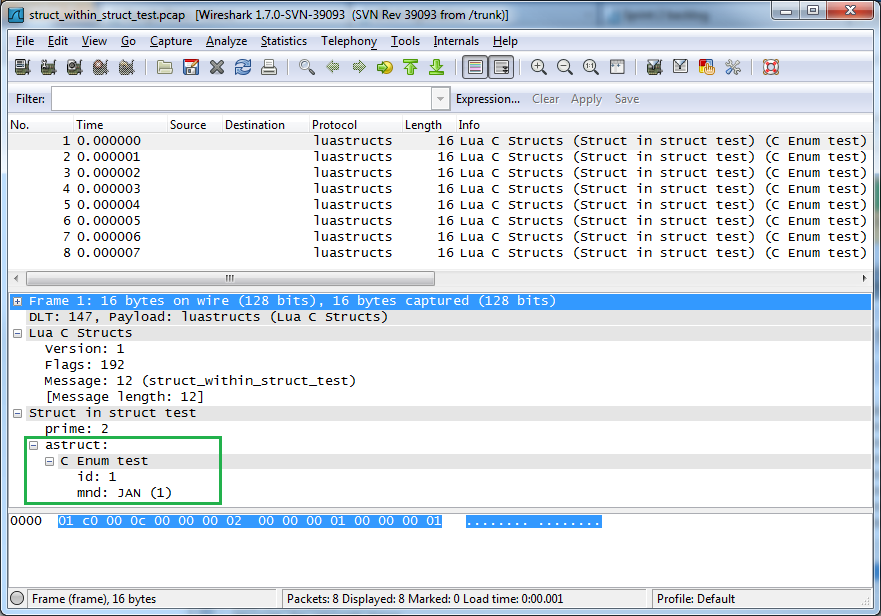
\includegraphics[width=\textwidth]{./sprints/img/wireshark_structwithstruct}
	\caption{Structs in Wireshark\label{fig:wsstructstruct}}
\end{figure}

\subsection{Support Enumerated Named Values}
%----------------------
In C there are two ways to do enumerations, the first option was explained in 
\autoref{sec:supportenum}, the other way is to use \#define which is shown in 
\autoref{code:defenum}. The advantage of using \#define is that the values 
can be generated. Since this cannot be understood by the parser, it can be 
generated directly from the header file, so it have to be supported by 
configuration. \autoref{code:enumconf}. The Lua-dissector will display the 
enum in the same way as in \autoref{sec:supportenum}.

\lstset{language=C,caption={Enumerated named values},label=code:defenum}
\lstinputlisting[language=C]{./sprints/code/def_enum.h}

\lstset{language=C,caption={Enumerated named values config},label=code:enumconf}
\lstinputlisting[language=C]{./sprints/code/def_enum.yml}

\subsection{Support for Bit Strings}
%----------------------
All bits in a basic data type can represent different values. An integer is 
represented by 4 bytes(32 bits), each of these bits can for example represent 
32 ''true/false' values. Our utility support configuration of these bits. Bits 
can be in groups, so they can represent more than two values. 
\autoref{code:bitstring} shows how bit string can be configured. 
\autoref{fig:wsbitstring} shows an example of how bit strings are displayed in 
Wireshark. Each group of bits are masked, so it is easier to see the values. 
The values are also named, if they are configured.

\begin{figure}[ht]
	\center
	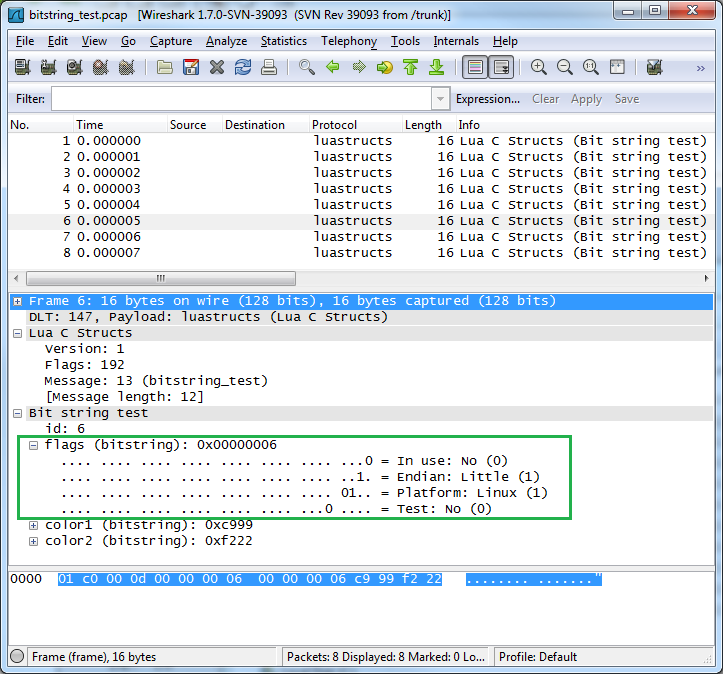
\includegraphics[width=\textwidth]{./sprints/img/wireshark_bitstring}
	\caption{Bit string in Wireshark\label{fig:wsbitstring}}
\end{figure}

\lstset{language=C,caption={Bitstring configuration},label=code:bitstring}
\lstinputlisting[language=C]{./sprints/code/bitstring.yml}

\subsection{Support Members of Type Array}
%----------------------
Csjark supports header-files with arrays, and is able to display them in 
Wireshark with the Lua-dissector. Csjark supports arrays of all data types 
implemented so far. The Wireshark dissector can display multidimensional 
arrays, and will create a new subtree for each dimension.  A representation of 
arrays in wireshark is displayed in \autoref{fig:wsarray}.

\begin{figure}[ht]
	\center
	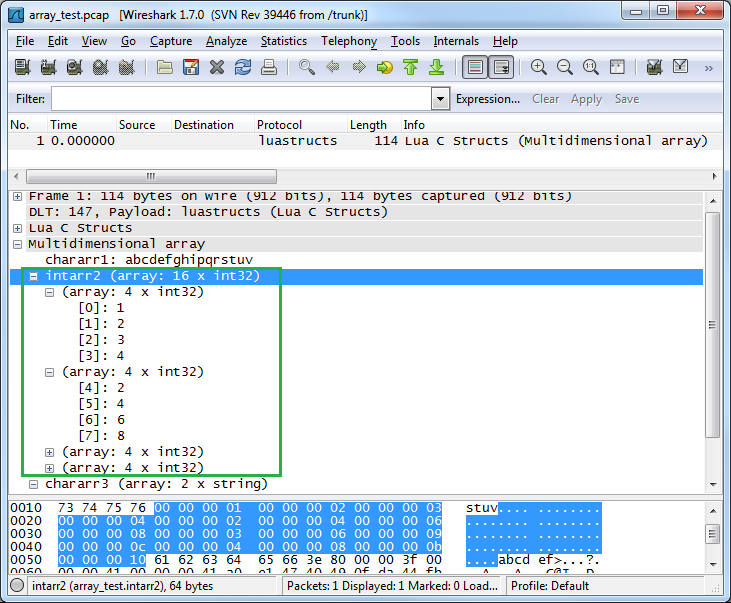
\includegraphics[width=\textwidth]{./sprints/img/wireshark_array}
	\caption{Arrays in Wireshark\label{fig:wsarray}}
\end{figure}

\subsection{Struct with Various Trailers}
%----------------------
The utility is able to support struct that has various trailers. Trailers are
data that follows a struct, this can be any kind of data. The utility is able to configure these data.
TODO: Not finished(add example + screenshot)

\subsection{Custom Lua Configuration}
%----------------------
Csjark can support custom Lua configuration, by including Lua-scripts from a file specified in the configuration file. This is implemented so that the users of the utility can include parts for the dissector, which our utility is not able to generate. The Lua-script can also include dissector for trailers, which are not from a struct.
TODO: Not finished(add example + screenshot)

\subsection{Dissector ID}
%----------------------
All struct-packets that Wireshark captures, has a header, one of the fields in 
the header is the message id. This id is used to load the the correct 
dissector when a packet is captured. Each dissector should have a unique id, 
to avoid possible conflicts. This functionallity is implemented and the 
message id must be specified in the configuration file, \autoref{code:msgid} 
is an example of how this is done.

\lstset{language=C,caption={Dissector ID config},label=code:msgid}
\lstinputlisting[language=C]{./sprints/code/messageid.yml}

\subsection{Endian Handling}
%----------------------
Endian handling is postponed to the next sprint, because it is a platform 
specific problem, and should be implemented together with platform support.

\subsection{Folder Support in the CLI}
%----------------------
Folder support in the CLI\footnote{Command-line Interface} has been 
implemented, so it is possible to generate Lua-scripts for all structs stored 
in a given folder. At the moment, all dissectors will be regenerated. 
Functionality to only generate modified or new header-files will be added in 
the next sprint. \autoref{fig:csjarkfolder} is an example usage of CSjark where
the command first shows the usage of CSjark, and the second command 
generates dissectors from the folder ''header/'' and configurations from ''etc/''.

\begin{figure}[ht]
	\center
	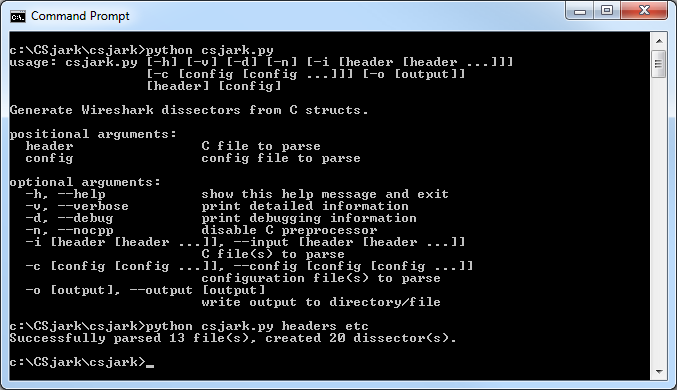
\includegraphics[width=\textwidth]{./sprints/img/csjark_folder}
	\caption{Arrays in Wireshark\label{fig:csjarkfolder}}
\end{figure}

\subsection{Support Custom Handling of Specified Data Types}
%----------------------
The utility supports custom handling of different data types, this includes 
functionality to support  time\_t and nstime\_t. All basic data types and 
struct members can be configured to be handled in a special way. 
\autoref{code:customstruct} show an example of a struct with four members, two 
of them are time fields, and the last two is a BOOL and an integer to be 
handled in a custom way. This struct is configured in 
\autoref{code:customconfig}, in the config the two time fields are configured 
to be respectively absolute time and relative time, and the BOOL type to have 
a size of four bytes. The struct member ''all' is configured with an enumerated 
value, and will be visible as a hex-value. \autoref{fig:customdatatype} is a 
screenshot of the struct in Wireshark.

\begin{figure}[ht]
	\center
	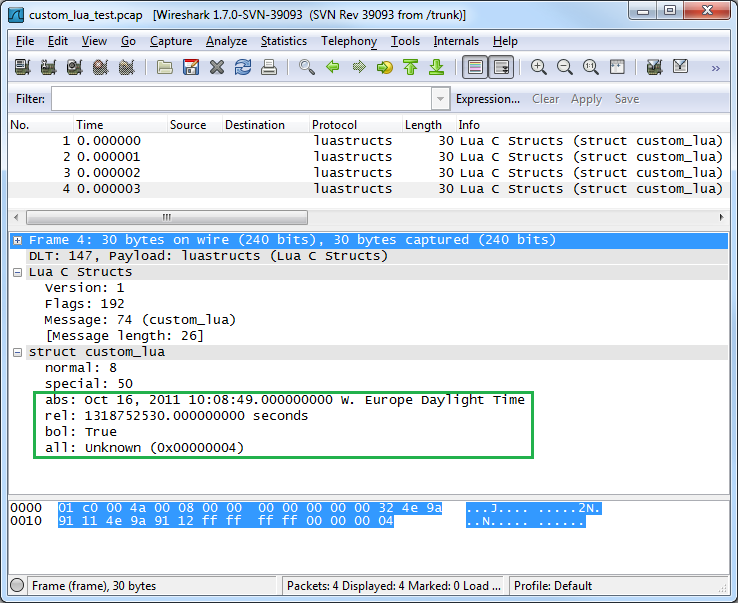
\includegraphics[width=\textwidth]{./sprints/img/wireshark_custom}
	\caption{Custom handling of Data Typesk\label{fig:customdatatype}}
\end{figure}

\lstset{language=C,caption={Struct for custom handling},label=code:customstruct}
\lstinputlisting[language=C]{./sprints/code/customfield.h}

\lstset{language=C,caption={Config for custom handling},label=code:customconfig}
\lstinputlisting[language=C]{./sprints/code/customfield.yml}

\subsection{Typedef Support}
%----------------------
Csjark is supporting the keyword typedef, which is a facility to create new 
data types names. \autoref{code:typedef} shows examples of typedef's that 
csjark supports.

\lstset{language=C,caption={Typedef example},label=code:typedef}
\lstinputlisting[language=C]{./sprints/code/typedef.h}

%-----------------------
\section{Sprint Testing}
%-----------------------
This section introduces the tests preformed during the sprint and their results. For sprint 2 it was also decided that the larger unit tests should also be documented and added to the test documents.

%subsection{Tests}
During the sprint the team executed a total of 6 tests with names as seen below. Tests executed:
\begin{itemize}
	\item TID08 - Supporting members of type enum \autoref{tab:sp2TID08}
	\item TID09 - Supporting members of type array  \autoref{tab:sp2TID09}
	\item TID10 - Supporting the display of structs within structs  \autoref{tab:sp2TID10}
	\item TID11 - Supporting enumerated named values  \autoref{tab:sp2TID11}
	\item TID12 - Supporting bit strings  \autoref{tab:sp2TID12}
	\item TID13 - Supporting structs with various trailers \autoref{tab:sp2TID13}
\end{itemize}

\subsection{Test Results}
%----------------------------
\begin{table}[!htb] \footnotesize \center
\caption{Recognizing Supporting enums \label{tab:sp2TID08}}
\begin{tabular}{l l}
	\toprule
	Header & Description \\
	\midrule
	Description &  Supporting members of type enum  \\
	Tester & Lars Solvoll Tønder \\
	Date & 15.10.2011 \\
	Result & Success\\
	\bottomrule
\end{tabular}
\end{table}

\begin{table}[!htb] \footnotesize \center
\caption{Recognizing Supporting arrays \label{tab:sp2TID09}}
\begin{tabular}{l l}
	\toprule
	Header & Description \\
	\midrule
	Description &  Supporting members of type array   \\
	Tester & Lars Solvoll Tønder \\
	Date & 15.10.2011 \\
	Result & Success\\
	\bottomrule
\end{tabular}
\end{table}


\subsection{Test Evaluation}
%-------------------------------

\subsubsection{Test Coverage}


%--------------------------
\section{Customer Feedback}
%--------------------------


%--------------------------
\section{Sprint Evaluation}
%--------------------------


